%!TEX root = /Users/stefano/Documents/Bonsai Club/TWBC/twbc.tex

\headline{\textbf{\Large\sffamily Bonsai Roots:}\\ 
{\textbf{\large\sffamily Meet the Members of TWBC}}}
\label{2025-05-roots}
\noindent
In each edition of \emph{Bonsai Roots,} we take a moment to step away from the pots and pruning and focus on the people who make our club such a vibrant community. Through their unique stories and passions, we see the many paths that lead to bonsai. This month, we're delighted to introduce \textbf{Mark Angold!}

\begin{itemize} 
    \item \textbf{What's your name and where in the country do you live?}

    \emph{I'm Mark Angold, and I live in Basingstoke.}

    \item \textbf{What are your favourite species of tree and why?}

    \emph{Pines, larches, and oaks --- all wonderful species native to the British Isles, which makes working with them feel deeply connected to our landscape.}

    \item \textbf{What aspect of bonsai do you enjoy?}

    \emph{The learning process. I enjoy striving to improve a little bit each and every day.}

    \item \textbf{What aspects of bonsai do you find most challenging?}

    \emph{Other people!} (He smiles.)

    \item \textbf{Who or what inspires you throughout your bonsai journey?}

    \emph{My wife who is endlessly supportive, Caroline Scott (Bonsai Caz) who is truly amazing; and of course, nature itself --- mountains, quiet moments, and peaceful places all inspire me.}

    \begin{window}[2,l,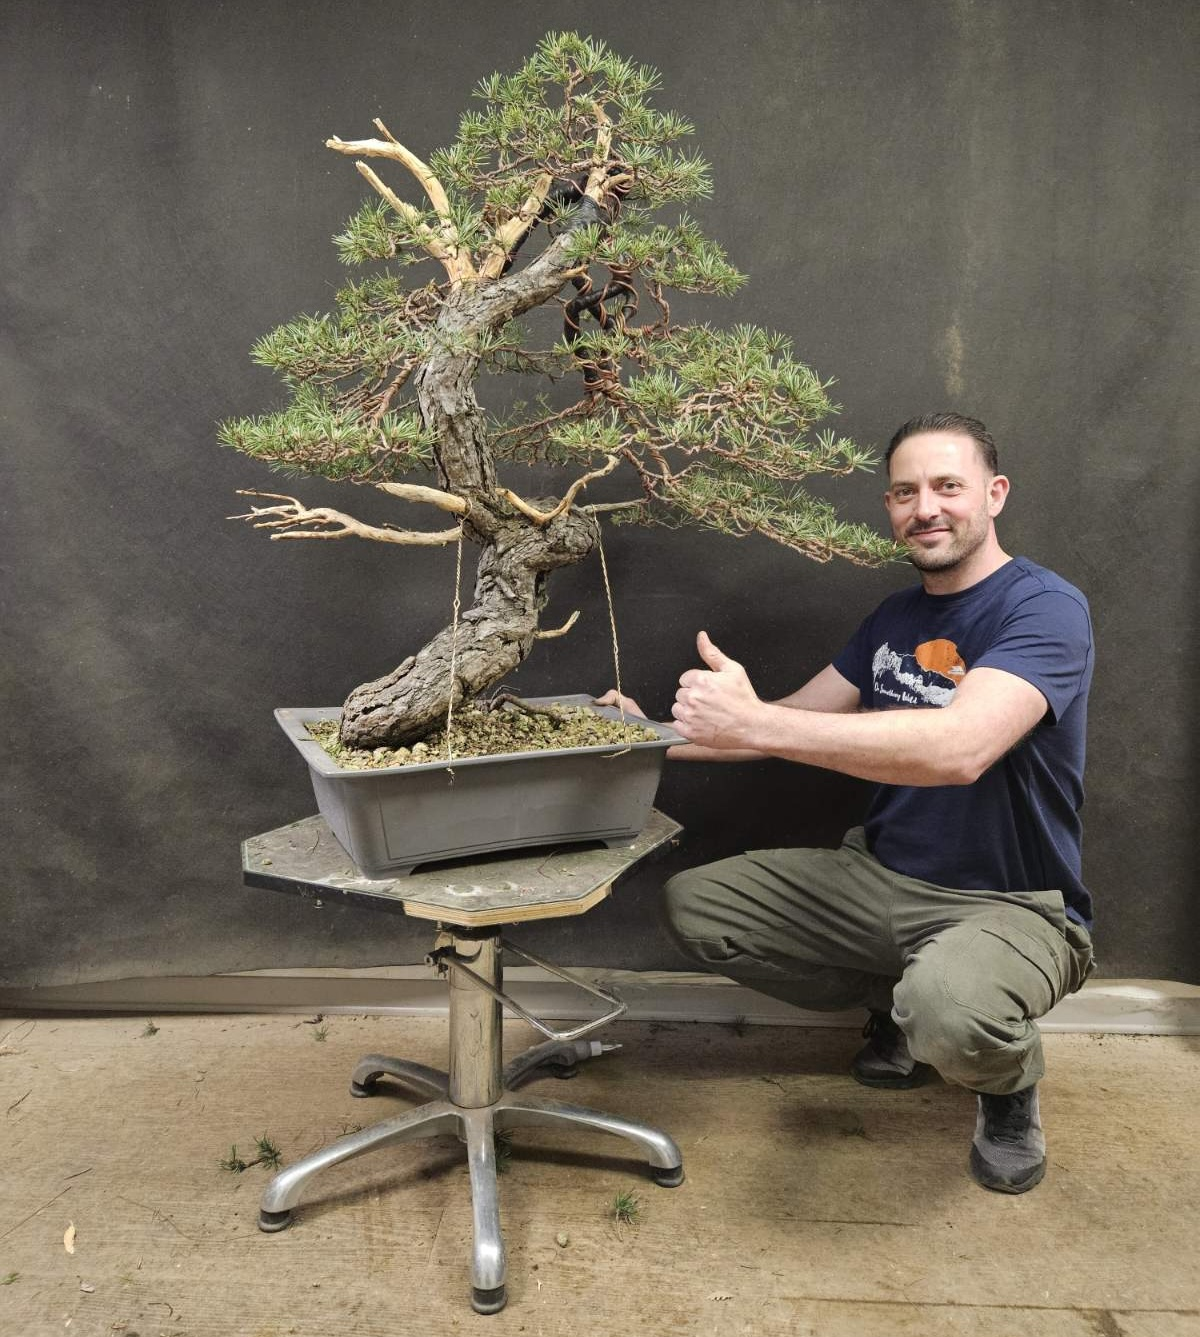
\includegraphics[width=1.0\columnwidth]{2025_05/res/roots_mark_angold.jpg},\centerline{\emph{Mark posing next to a wonderful specimen of Scott's pine.}}]
    \end{window}
    \columnbreak
    
        \item \textbf{How long have you been interested in keeping bonsai?}

    \emph{For about four and a half years. It's been a steady and rewarding journey of discovery since then.}

    \item \textbf{What stimulated your interest in bonsai?}

    \emph{After heart surgery, I needed something to help me find peace and focus. Bonsai quickly became the perfect way to bring calm into my life.}

    \item \textbf{If you could give someone new to bonsai any tips, what would it be?}

    \emph{Take time choosing good material — it's far better to start with potential than to struggle with trees that won't ever amount to much.}

    \item \textbf{Why do you enjoy being part of TWBC, and do you have any ideas or suggestions for the club's future?}

    \emph{I've really enjoyed my experience so far. The members are welcoming and knowledgeable, and I'm excited to keep learning and helping where I can.}

    \item \textbf{One word to describe what bonsai means to you?}

    \emph{Everything.}

    \item \textbf{What are your future goals regarding your own trees and learning more about the hobby?}

    \emph{I'd love to help spread good bonsai across England and beyond. I'm committed to doing bonsai for life and pushing myself to get better every year.}

    \item \textbf{How would you like to see your bonsai journey progress in the future?}

    \emph{I hope to travel and learn from other countries, but my focus will always stay rooted in helping English bonsai grow stronger.}
\end{itemize}

Thank you, Mark, for sharing your heartfelt story and passion. We can't wait to see where your bonsai journey takes you next. Join us next month for another glimpse into the lives behind the trees in \emph{Bonsai Roots}!

\begin{center}
    $\cdots$
\end{center}

\noindent
\emph{If you are a novice member of the club and you'd like to be featured in a future edition of Bonsai Roots, please fill in the form at \href{https://forms.gle/quVXa4L8rhpnT5kr6}{this address}! We're always eager to share the stories of our wonderful members.}

\closearticle 
\columnbreak